% Practice Test 03 — Indiana Edition
% Questions: 30 (21 MC + 9 SA)
% Generated by scripts/generate_practice_tests.py

\begin{practiceQuestion}{1-3-q29}{gsa}
\begin{questionText}
The graph shows a proportional relationship. Use the labeled point to find $k$, then determine $y$ when $x = 12$.

\begin{center}
\begin{tikzpicture}[scale=0.6]
  \draw[step=1,gray!20,thin] (0,0) grid (8,8);
  \draw[thick,->] (0,0) -- (8.5,0) node[right]{\small $x$};
  \draw[thick,->] (0,0) -- (0,8.5) node[above]{\small $y$};
  \foreach \x in {2,4,6,8} \draw (\x,0.07) -- (\x,-0.07) node[below]{\tiny \x};
  \foreach \y in {2,4,6,8} \draw (0.07,\y) -- (-0.07,\y) node[left]{\tiny \y};
  \draw[thick,funBlue] (0,0) -- (8,6);
  \fill[funBlue] (0,0) circle (2.5pt);
  \fill[funBlue] (4,3) circle (2.5pt) node[above left]{\small $(4, 3)$};
\end{tikzpicture}
\end{center}
\end{questionText}
\correctAnswer{$k = 0.75$; when $x = 12$, $y = 9$}
\explanation{$k = \frac{3}{4} = 0.75$. Then $y = 0.75 \times 12 = 9$.}
\end{practiceQuestion}

\begin{practiceQuestion}{1-5-q12}{mc}
\begin{questionText}
A graph passes through $(5, 12.5)$. What is $x$ when $y = 40$?
\end{questionText}
\choiceA{$10$}
\choiceB{$12$}
\choiceC{$16$}
\choiceD{$20$}
\correctAnswer{C}
\explanation{$k = \frac{12.5}{5} = 2.5$, so $y = 2.5x$. When $y = 40$: $40 = 2.5x$, giving $x = 16$.}
\end{practiceQuestion}

\begin{practiceQuestion}{1-6-q11}{mc}
\begin{questionText}
A train travels $315$ miles in $4.5$ hours. At this rate, how far does it travel in $7$ hours?
\end{questionText}
\choiceA{$420$ miles}
\choiceB{$455$ miles}
\choiceC{$490$ miles}
\choiceD{$525$ miles}
\correctAnswer{C}
\explanation{Rate: $315 \div 4.5 = 70$ mph. In $7$ hours: $70 \times 7 = 490$ miles.}
\end{practiceQuestion}

\begin{practiceQuestion}{2-2-q25}{sa}
\begin{questionText}
A farmer harvested $420$ apples. He sold $315$ of them. What percent did he sell?
\end{questionText}
\correctAnswer{$75\%$}
\explanation{$\frac{315}{420} = \frac{p}{100}$. Cross-multiply: $420p = 31{,}500$. Divide: $p = 75\%$.}
\end{practiceQuestion}

\begin{practiceQuestion}{2-5-q26}{gmc}
\begin{questionText}
The table shows the monthly sales and commission rates for three employees. Who earned the most commission?

\begin{center}
\begin{tabular}{|l|c|c|}
\hline
\textbf{Employee} & \textbf{Sales} & \textbf{Commission Rate} \\
\hline
Alex & $\$5{,}000$ & $6\%$ \\
\hline
Brenda & $\$8{,}000$ & $4\%$ \\
\hline
Carlos & $\$6{,}000$ & $5\%$ \\
\hline
\end{tabular}
\end{center}
\end{questionText}
\choiceA{Alex ($\$300$)}
\choiceB{Brenda ($\$320$)}
\choiceC{Carlos ($\$300$)}
\choiceD{Alex and Carlos are tied ($\$300$ each)}
\correctAnswer{B}
\explanation{Alex: $5{,}000 \times 0.06 = \$300$. Brenda: $8{,}000 \times 0.04 = \$320$. Carlos: $6{,}000 \times 0.05 = \$300$. Brenda earned the most.}
\end{practiceQuestion}

\begin{practiceQuestion}{2-7-q18}{mc}
\begin{questionText}
A package was estimated to weigh $10$ kg, but it actually weighs $12$ kg. A second package was estimated to weigh $50$ kg, but it actually weighs $52$ kg. Which estimate has the smaller percent error?
\end{questionText}
\choiceA{The first package}
\choiceB{The second package}
\choiceC{They have the same percent error}
\choiceD{Cannot be determined}
\correctAnswer{B}
\explanation{First: $\frac{2}{12} \times 100 \approx 16.7\%$. Second: $\frac{2}{52} \times 100 \approx 3.8\%$. The second has a smaller percent error.}
\end{practiceQuestion}

\begin{practiceQuestion}{3-1-q26}{gmc}
\begin{questionText}
Use the number line below. Which point represents $-3$?

\begin{center}
\begin{tikzpicture}
  \draw[thick,->] (-5.5,0) -- (5.5,0);
  \foreach \x in {-5,...,5} \draw (\x,0.1) -- (\x,-0.1) node[below] {$\x$};
  \fill[funRed] (-3,0) circle (4pt) node[above=6pt] {A};
  \fill[funBlue] (1,0) circle (4pt) node[above=6pt] {B};
  \fill[funGreen] (-1,0) circle (4pt) node[above=6pt] {C};
  \fill[funOrange] (3,0) circle (4pt) node[above=6pt] {D};
\end{tikzpicture}
\end{center}
\end{questionText}
\choiceA{Point A}
\choiceB{Point B}
\choiceC{Point C}
\choiceD{Point D}
\correctAnswer{A}
\explanation{Point A is located at $-3$ on the number line.}
\end{practiceQuestion}

\begin{practiceQuestion}{3-2-q19}{sa}
\begin{questionText}
What is $(-16) + 9$?
\end{questionText}
\correctAnswer{$-7$}
\explanation{Different signs: $16 - 9 = 7$. The larger absolute value ($16$) is negative, so the answer is $-7$.}
\end{practiceQuestion}

\begin{practiceQuestion}{4-2-q12}{mc}
\begin{questionText}
Simplify $-6y + 4y - y$.
\end{questionText}
\choiceA{$-3y$}
\choiceB{$-y$}
\choiceC{$3y$}
\choiceD{$-11y$}
\correctAnswer{A}
\explanation{$-6y + 4y = -2y$. Then $-2y - y = -3y$.}
\end{practiceQuestion}

\begin{practiceQuestion}{4-3-q11}{mc}
\begin{questionText}
Expand and simplify $3(x - 2) + 2(x + 4)$.
\end{questionText}
\choiceA{$5x + 2$}
\choiceB{$5x - 2$}
\choiceC{$5x + 14$}
\choiceD{$x + 2$}
\correctAnswer{A}
\explanation{Expand each: $3x - 6 + 2x + 8$. Combine: $(3x + 2x) + (-6 + 8) = 5x + 2$.}
\end{practiceQuestion}

\begin{practiceQuestion}{5-4-q16}{mc}
\begin{questionText}
A student estimates that the solution to $0.48x + 3.1 = 12.7$ is about $x = 20$. Is this estimate reasonable?
\end{questionText}
\choiceA{Yes, the exact answer is $20$}
\choiceB{Yes, the exact answer is close to $20$}
\choiceC{No, the exact answer is about $10$}
\choiceD{No, the exact answer is about $33$}
\correctAnswer{A}
\explanation{Subtract $3.1$: $0.48x = 9.6$. Divide by $0.48$: $x = 20$. The estimate is exactly correct.}
\end{practiceQuestion}

\begin{practiceQuestion}{5-5-q13}{mc}
\begin{questionText}
Which value of $x$ is a solution to $4x - 1 > 11$?
\end{questionText}
\choiceA{$x = 2$}
\choiceB{$x = 3$}
\choiceC{$x = 4$}
\choiceD{$x = 1$}
\correctAnswer{C}
\explanation{Solve: $4x > 12$, so $x > 3$. Only $x = 4$ satisfies $x > 3$. Check: $4(4) - 1 = 15 > 11$ \checkmark.}
\end{practiceQuestion}

\begin{practiceQuestion}{5-6-q02}{mc}
\begin{questionText}
Which graph represents $x \leq -2$?
\end{questionText}
\choiceA{Open circle at $-2$, shade left}
\choiceB{Closed circle at $-2$, shade right}
\choiceC{Closed circle at $-2$, shade left}
\choiceD{Open circle at $-2$, shade right}
\correctAnswer{C}
\explanation{$x \leq -2$: closed circle (includes $-2$) and shade left (values less than or equal to $-2$).}
\end{practiceQuestion}

\begin{practiceQuestion}{6-1-q05}{mc}
\begin{questionText}
A scale drawing uses $1$ cm $= 4$ m. A room is $5$ cm by $3$ cm on the drawing. What is the actual area of the room?
\end{questionText}
\choiceA{$15$ m$^2$}
\choiceB{$60$ m$^2$}
\choiceC{$192$ m$^2$}
\choiceD{$240$ m$^2$}
\correctAnswer{D}
\explanation{Actual dimensions: $5 \times 4 = 20$ m and $3 \times 4 = 12$ m. Area: $20 \times 12 = 240$ m$^2$.}
\end{practiceQuestion}

\begin{practiceQuestion}{6-3-q27}{gmc}
\begin{questionText}
The diagram shows a triangle with the given measurements. How many different triangles can be drawn with these exact conditions?

\begin{center}
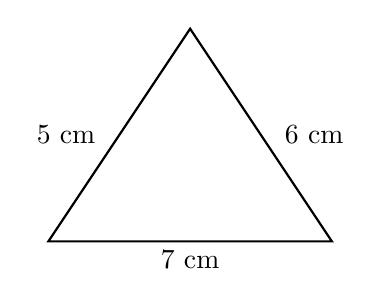
\begin{tikzpicture}[scale=0.9]
  \draw[thick] (0,0) -- (4,0) -- (2,3) -- cycle;
  \node[below] at (2,0) {$7$ cm};
  \node[left] at (0.8,1.5) {$5$ cm};
  \node[right] at (3.2,1.5) {$6$ cm};
\end{tikzpicture}
\end{center}
\end{questionText}
\choiceA{None}
\choiceB{Exactly one}
\choiceC{Exactly two}
\choiceD{Infinitely many}
\correctAnswer{B}
\explanation{Three side lengths that satisfy the triangle inequality (SSS) produce exactly one unique triangle. Check: $5 + 6 = 11 > 7$, $5 + 7 = 12 > 6$, $6 + 7 = 13 > 5$. All pass.}
\end{practiceQuestion}

\begin{practiceQuestion}{6-4-q20}{sa}
\begin{questionText}
Can a triangle have sides $8$, $8$, and $16$? Explain.
\end{questionText}
\correctAnswer{No}
\explanation{$8 + 8 = 16$, which is not greater than $16$. The triangle inequality requires the sum to be strictly greater.}
\end{practiceQuestion}

\begin{practiceQuestion}{6-5-q25}{sa}
\begin{questionText}
A square pyramid has a base edge of $8$ cm. It is sliced parallel to the base halfway up. Is the cross-section larger, smaller, or the same size as the base?
\end{questionText}
\correctAnswer{Smaller than the base}
\explanation{A horizontal cut parallel to the base of a pyramid produces a similar shape that is smaller than the base. Halfway up, the cross-section is a $4$ cm square (half the edge length).}
\end{practiceQuestion}

\begin{practiceQuestion}{6-6-q01}{mc}
\begin{questionText}
Two angles are supplementary. One angle is $115°$. What is the other angle?
\end{questionText}
\choiceA{$25°$}
\choiceB{$55°$}
\choiceC{$65°$}
\choiceD{$75°$}
\correctAnswer{C}
\explanation{Supplementary angles sum to $180°$. $180° - 115° = 65°$.}
\end{practiceQuestion}

\begin{practiceQuestion}{6-7-q05}{mc}
\begin{questionText}
Which transformation changes the position of a figure without changing its size, shape, or orientation?
\end{questionText}
\choiceA{Reflection}
\choiceB{Rotation}
\choiceC{Translation}
\choiceD{Dilation}
\correctAnswer{C}
\explanation{A translation (slide) moves every point the same distance and direction. The figure keeps its size, shape, and orientation.}
\end{practiceQuestion}

\begin{practiceQuestion}{7-3-q06}{mc}
\begin{questionText}
A circular tablecloth covers a table with a diameter of $4$ feet. What is the area of the tablecloth? Use $\pi \approx 3.14$.
\end{questionText}
\choiceA{$12.56$ ft$^2$}
\choiceB{$25.12$ ft$^2$}
\choiceC{$50.24$ ft$^2$}
\choiceD{$6.28$ ft$^2$}
\correctAnswer{A}
\explanation{$r = 4 \div 2 = 2$ ft. $A = \pi r^2 = 3.14 \times 4 = 12.56$ ft$^2$.}
\end{practiceQuestion}

\begin{practiceQuestion}{7-4-q30}{gsa}
\begin{questionText}
The figure below shows a rectangle with a circular hole. What is the area of the shaded region? Use $\pi \approx 3.14$.

\begin{center}
\begin{tikzpicture}[scale=0.4]
  \fill[funBlue!20] (0,0) rectangle (12,8);
  \fill[white] (6,4) circle (2);
  \draw[thick,funBlue] (0,0) rectangle (12,8);
  \draw[thick,funRed] (6,4) circle (2);
  \draw[thick,funRed,<->] (0,-0.8) -- (12,-0.8);
  \node[below,funRed] at (6,-0.8) {$12$ cm};
  \draw[thick,funRed,<->] (-0.8,0) -- (-0.8,8);
  \node[left,funRed] at (-0.8,4) {$8$ cm};
  \draw[thick,funRed,<->] (6,4) -- (8,4);
  \node[above,funRed] at (7,4) {$3$ cm};
\end{tikzpicture}
\end{center}
\end{questionText}
\correctAnswer{$67.74$ cm$^2$}
\explanation{Rectangle: $12 \times 8 = 96$ cm$^2$. Circle: $\pi r^2 = 3.14 \times 9 = 28.26$ cm$^2$. Shaded region: $96 - 28.26 = 67.74$ cm$^2$.}
\end{practiceQuestion}

\begin{practiceQuestion}{7-5-q14}{mc}
\begin{questionText}
A rectangular prism is $6$ ft by $6$ ft by $10$ ft. What is its surface area?
\end{questionText}
\choiceA{$72$ ft$^2$}
\choiceB{$240$ ft$^2$}
\choiceC{$312$ ft$^2$}
\choiceD{$360$ ft$^2$}
\correctAnswer{C}
\explanation{$SA = 2(6 \times 6) + 2(6 \times 10) + 2(6 \times 10) = 72 + 120 + 120 = 312$ ft$^2$.}
\end{practiceQuestion}

\begin{practiceQuestion}{7-6-q02}{mc}
\begin{questionText}
Which formula is used to find the volume of any prism?
\end{questionText}
\choiceA{$V = lwh$ only}
\choiceB{$V = Bh$}
\choiceC{$V = 2(lw + lh + wh)$}
\choiceD{$V = \frac{1}{3}Bh$}
\correctAnswer{B}
\explanation{The general formula for the volume of any prism is $V = Bh$, where $B$ is the area of the base and $h$ is the height.}
\end{practiceQuestion}

\begin{practiceQuestion}{8-1-q24}{sa}
\begin{questionText}
A random sample of $100$ out of $4{,}000$ residents found that $45$ support a new library. Predict how many residents support it.
\end{questionText}
\correctAnswer{$1{,}800$}
\explanation{$\frac{45}{100} = 45\%$. Then $45\%$ of $4{,}000 = 1{,}800$.}
\end{practiceQuestion}

\begin{practiceQuestion}{8-3-q19}{sa}
\begin{questionText}
Group A: mean $65$, MAD $5$. Group B: mean $75$, MAD $5$. How many MADs apart are the means?
\end{questionText}
\correctAnswer{$2$ MADs}
\explanation{Difference: $75 - 65 = 10$. Divide by MAD: $\frac{10}{5} = 2$ MADs.}
\end{practiceQuestion}

\begin{practiceQuestion}{8-4-q04}{mc}
\begin{questionText}
Which measure of variability focuses on the middle $50\%$ of the data?
\end{questionText}
\choiceA{Range}
\choiceB{Mean}
\choiceC{Interquartile range (IQR)}
\choiceD{Median}
\correctAnswer{C}
\explanation{IQR $= Q_3 - Q_1$ measures the spread of the middle $50\%$ of the data.}
\end{practiceQuestion}

\begin{practiceQuestion}{8-7-q13}{mc}
\begin{questionText}
A line graph shows a company's profits: Q1 $\$50{,}000$, Q2 $\$60{,}000$, Q3 $\$55{,}000$, Q4 $\$70{,}000$. What was the increase from Q1 to Q4?
\end{questionText}
\choiceA{$\$10{,}000$}
\choiceB{$\$15{,}000$}
\choiceC{$\$20{,}000$}
\choiceD{$\$70{,}000$}
\correctAnswer{C}
\explanation{$\$70{,}000 - \$50{,}000 = \$20{,}000$.}
\end{practiceQuestion}

\begin{practiceQuestion}{9-4-q27}{gmc}
\begin{questionText}
The table shows a probability model for a spinner. The spinner is spun $100$ times and the results are shown. Does the observed data support the model?

\begin{center}
\begin{tabular}{|c|c|c|}
\hline
\textbf{Color} & \textbf{Model $P$} & \textbf{Observed Frequency} \\
\hline
Red & $0.40$ & $38$ \\
\hline
Blue & $0.35$ & $36$ \\
\hline
Yellow & $0.25$ & $26$ \\
\hline
\end{tabular}
\end{center}
\end{questionText}
\choiceA{No, the data is very different from the model}
\choiceB{Yes, the observed frequencies are close to the predicted values}
\choiceC{No, because Red appeared fewer times than predicted}
\choiceD{The model cannot be checked with only $100$ spins}
\correctAnswer{B}
\explanation{Predicted: Red $= 40$, Blue $= 35$, Yellow $= 25$. Observed: $38$, $36$, $26$. These are close, supporting the model.}
\end{practiceQuestion}

\begin{practiceQuestion}{9-6-q01}{mc}
\begin{questionText}
What is the probability of flipping two coins and getting heads on both?
\end{questionText}
\choiceA{$\frac{1}{2}$}
\choiceB{$\frac{1}{3}$}
\choiceC{$\frac{1}{4}$}
\choiceD{$\frac{3}{4}$}
\correctAnswer{C}
\explanation{Sample space: HH, HT, TH, TT ($4$ outcomes). Only HH is heads-heads. $P = \frac{1}{4}$.}
\end{practiceQuestion}

\begin{practiceQuestion}{9-7-q20}{sa}
\begin{questionText}
You roll a die $90$ times to simulate a $\frac{1}{6}$ probability event. How many times do you expect the event to occur?
\end{questionText}
\correctAnswer{$15$}
\explanation{$90 \times \frac{1}{6} = 15$.}
\end{practiceQuestion}
